\documentclass{article}


\usepackage{arxiv}

\usepackage[utf8]{inputenc} % allow utf-8 input
\usepackage[T1]{fontenc}    % use 8-bit T1 fonts
\usepackage{hyperref}       % hyperlinks
\usepackage{url}            % simple URL typesetting
\usepackage{booktabs}       % professional-quality tables
\usepackage{amsfonts}       % blackboard math symbols
\usepackage{nicefrac}       % compact symbols for 1/2, etc.
\usepackage{microtype}      % microtypography
\usepackage{lipsum}
\usepackage{graphicx}

\title{High Temperature Superconductors and their applications}


\author{
	Anshul ~Yadav\thanks{This paper has been submitted by Anshul Yadav (Entry No. 2017EE10565, Webpage: \href{http://anshulyadav.me}{http://anshulyadav.me}) as Termpaper for PYL102.} \\
	Department of Electrical Engineering\\
	Indian Institute of Technology Delhi\\
	Delhi, India 110016 \\
	\texttt{ee1170565@iitd.ac.in} \\
	%% examples of more authors
	%   \And
	%  Elias D.~Striatum \\
	%   Department of Electrical Engineering\\
	%   Mount-Sheikh University\\
	%   Santa Narimana, Levand \\
	%   \texttt{stariate@ee.mount-sheikh.edu} \\
	%% \AND
	%% Coauthor \\
	%% Affiliation \\
	%% Address \\
	%% \texttt{email} \\
	%% \And
	%% Coauthor \\
	%% Affiliation \\
	%% Address \\
	%% \texttt{email} \\
	%% \And
	%% Coauthor \\
	%% Affiliation \\
	%% Address \\
	%% \texttt{email} \\
}

\begin{document}
	\maketitle
	
	\begin{abstract}
		High temperature superconductivity, discovered by \emph{Bednorz et al.}  (IBM,1986) remains an active area of research worldwide, because of its high $T_c$. The search for new superconductors has been sparked off after this discovery. High Temperature Superconductors (referred to also as HTS or high-$T_c$ superconductors) have found demonstrated application in a vast variety of applications due to its high power density and high efficiency.  In areas like power electronics, HTS has been already used for prototypes of power cables, transformers, motors, and fault current limiters. HTS have found profound applications in scientific magnets and filters and in NMR and MRI techniques. However full-fledged commercialization of these applications is not yet observed. This paper briefly describes High Temperature semiconductors, current developments on it and its major applications. 
	\end{abstract}
	
	
	% keywords can be removed
	\keywords{High Temperature Superconductors \and HTS Applications}
	
	
	\section{Introduction}
	Superconductors are materials which have exactly zero electrical resistance, and magnetic flux lines are expulsed out. Considering the Bardeen–Cooper–Schrieffer theory (BCS theory) to be valid and defining the Transition temperature as the temperature at which the electrical resistivity of the material drops to zero, we review the development of HTS and its applications. The ordinary superconductors require very low temperatures such as 30 K which are very difficult to achieve for all commercial purposes. The discovery of High Temperature superconductors by  Georg Bednorz and K. Alex Müller in 1986 at IBM  which can go as high as 250K \cite{highestTc} paved its way for commercial applications. Superconductors are definitely at an advantage with extremely low losses and high current carrying capability they offer high power density and high efficiency. HTS has been proven to enable novel devices like Magnetic Energy Storage (SMES), magnetic bearings, fault current limiters and switches\cite{HTSdevices}. HTS has seen large number of applications in Power Electronics with established prototypes of power cables, \cite{powercable} transformers \cite{HTStransformer}, motors \cite{HTSmotor}, and SuperConducting Fault Current Limiters (SCFCL) \cite{SCFCL}.
	
	High temperature superconductors require liquid Nitrogen $(77 K)$ for cooling instead of the costlier liquid Helium $(4.2 K)$. Liquid Nitrogen has proved to be a cheap alternative and it is present in abundant quantity. It acts as a coolant and facilitates lower temperatures at which superconductivity is observed. Recent attempts to take this cooling temperature to room temperature have successfully demonstrated that this can be achieved using high pressure which is not yet useful for most of the practical applications. Another problem with HTS is that currently known semiconductors are ceramics which makes it very difficult to convert them into desired shapes and forces limited usability.
	
	
	
	\section{Superconductivity and Superconductors}
	\label{sec:headings}
	Superconductivity is the phenomenon of zero electrical resistivity and complete expulsion of the magnetic field from the material. Dutch physicist Heike Kamerlingh Onnes discovered it on April 8, 1911. The temperature at which the electrical resistivity drops to zero is known as \textbf{critical temperature} (abbreviated as $T_c$). This sudden transition appears to be a transition into a different phase of matter similar to Bose-Einstein Condensate (BEC). The disappearance of electrical resistivity was modeled in terms of electron pairing in the crystal lattice in theory proposed by John Bardeen, Leon Cooper, and John Robert Schrieffer in 1957, later known as \textbf{BCS Theory}. The phenomenon of expelling the magnetic field by the material when a transition occurs from normal phase to a superconducting phase is known as \textbf{Meissner effect}. We briefly review these two concepts below as they are essential in the understanding of superconductors.
	
	\subsection{BCS Theory and Cooper Pairs}
	We take a brief digression and recall that \textit{fermions} are pair of fundamental particles like electrons which follows Pauli's Exclusion principle and have half-integer multiples (e.g.,$ \pm 1/2, \pm 3/2, \pm 5/2 $, etc.) spins. There is another class of particles known as \textit{bosons} with spins in integer multiples (e.g.,$ 0, \pm 1, \pm 2$, etc.) which doesn't obey Pauli's Exclusion principle and can condense into same energy level. BCS theory proposed that electrons near the Fermi level pair up together to give \textbf{Cooper Pairs}. These coupled electrons are essentially bosons and condense into the ground state.  
	
	\begin{figure}[h]
		\centering
		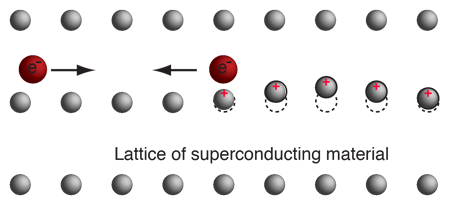
\includegraphics[width=8cm]{bcs7.png}
		\caption{A passing electron attracts the lattice, causing a slight ripple toward its path.}
		    \source{src: \href{http://hyperphysics.phy-astr.gsu.edu}{http://hyperphysics.phy-astr.gsu.edu}}
	\end{figure}
	
	\begin{figure}[h]
		\centering
		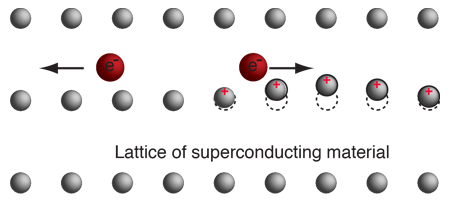
\includegraphics[width=8cm]{bcs8.png}
		\caption{Another electron passing in the opposite direction is attracted to that displacement.}
		    \source{src: \href{http://hyperphysics.phy-astr.gsu.edu}{http://hyperphysics.phy-astr.gsu.edu}}
	\end{figure}
	
	These coupled electrons become correlated, and at sufficiently low temperatures, many such pairs exist. These pairs strongly overlap with each other and form a \textit{condensed state}. At this stage, thermal vibrations and oscillations of atom are unable to break these overlappings and therefore no resistance is experienced by electron flow. 
	
	
	\subsection{Meissner Effect}
	Meissner effect is an important property observed by superconductors. It refers to the expulsion of magnetic fields from the superconductor. This is a direct consequence of the fact that magnetic field dies out after small penetration depth (commonly known as skin depth in Electromagnetics).
	$$
	\nabla^2 H = \gamma^2 H
	$$
	BCS Theory successfully explained the Meissner effect in superconductors and Bardeen, Cooper, and Schrieffer received Nobel Prize in 1957 for this theory. 
	
	\subsection{Critical Magnetic Field}
	The maximum field that can be applied without breaking the superconducting state at a given temperature is known as the Critical magnetic field (Sometimes critical field). There is a direct relation between critical field and critical current $-$ which is the maximum electric current density that can be carried by a superconductor \cite{criticalfieldform}. The critical field is an important parameter for high temperature superconductors as we will see later in this paper.
	
	\subsection{History of Superconductors}
	Although BCS Theory didn't put any constraint on critical temperature($T_c$), physicists used to believe that $30K$ is the upper limit for $T_c$, which is presumably false. Such low temperatures were reached using liquid Helium as a coolant which has boiling temperature as low as $4 K$. Until recently in 1986,  Bednorz and Müller discovered superconductivity in lanthanum-based cuprate perovskite material which increased the $T_c$ to $35 K$. This increase in the assumed limit of $T_c \approx 30$ led to massive research in finding semiconductors with high $T_c$. It was later found by Bednorz and Müller that by replacing Lanthanum with Yttrium raised critical temperature to $T_c = 92 K$ for which both of them jointly received Nobel Prize in 1987. This rise in critical temperature allowed $N_2$ as a coolant which is abundant in the atmosphere and readily available. 
	
	
	\section{High Temperature Superconductors} Various attempts have been made to achieve room temperature semiconductors. Eremets et al., (2018) claimed that they have achieved $T_c$ as high as $250 K$ in $H_2 S$ which is a leap forward to room temperature superconductivity. But the caveat here is that such high critical temperatures require very high pressure of the order of $170$ GPa's and this makes it practically unusable for commercial applications. But still, Eremets idea encourages new methods of superconductivity in which high oscillations are ascertained at high temperature in light materials and pressure keeps it intact. Like most of the other work in High Temperature superconductivity this work remains unverified. Further Eremets et al. was not able to show Meissner effect which is crucial to superconductors. Room temperature semiconductors are not far away from now. Gauging their new applications and commercializing them is underway.  
	
	\paragraph{}
	Another advantage of High Temperature superconductors is that they have high critical field and therefore high critical current density. This leads to their high current carrying capability and low resistivity allows high energy density and negligible energy losses. High Temperature Superconductors can revolutionize the world provided we can discover materials which can be easily transformed into wires/rods and desired shapes instead of current brittle ceramics which are costly and difficult to manufacture \cite{ceramicsbarrier}. It has been shown that the cost involved in maintaining HTS is lesser than the performance and efficiency achieved from them. Once we can form desired shapes and wires we would be able to achieve large scale commercialization of HTS applications.
	
	\begin{figure}[h]
		\centering
		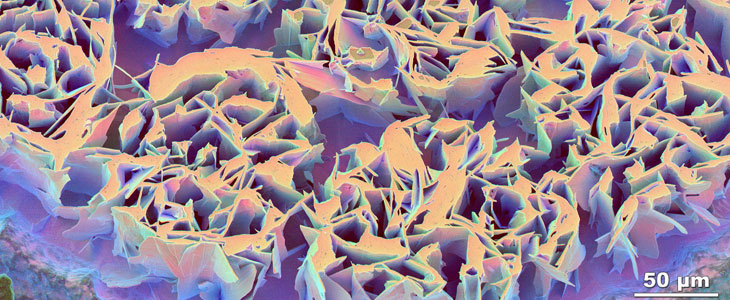
\includegraphics[width=16cm]{hts_etched_bi2212_nature_730.jpg}
		\caption{High density Bi-2212 filament macrostructure produced by the over-pressure (OP) technique developed at the Applied Superconductivity Center. Image: Peter Lee Courtesy: \href{https://nationalmaglab.org}{https://nationalmaglab.org}}
	\end{figure} 
	
	\paragraph{Recent Advances}
	The term high-temperature superconductor was used interchangeably with cuprate superconductor until Fe-based superconductors were discovered in 2008. The best known high-temperature superconductors at \textit{ambient pressure} are Bismuth Strontium Calcium Copper Oxide, BSCCO, and Yttrium Barium Copper Oxide, YBCO. Despite incredible properties of High Temperature Superconductors, scientists and researchers believe that new materials or a phenomenon like superconductivity may exist approaching room temperature, affordability, and practicality all at the same time. New materials are being discovered and steps have already been taken in this direction. The 2016 Nobel Prize in Physics was awarded for the theoretical work that characterizes topological insulators—materials that exhibit similarly strange quantum behaviors \cite{noblePress}. These materials can be considered perfect insulators for the bulk of the material but behave as extraordinarily good conductors on surface of these materials. Room-temperature superconductivity has remained an exciting field over a century, and researchers have proposed various materials and theories, but most of them remain either unverified or false claims. It is difficult to reproduce such results, and most of these claims remained for a trillionth of a second or so. With no upper bound on the critical temperature in BCS Theory, the existence of room temperature superconductivity remains yet to be ascertained.
	
	\section{Applications}
	Since its discovery, superconductivity has found large number of applications in diverse fields. Applications of superconductivity can be found in transportation (Maglev), marine and military (propulsion motors, degaussing systems and Electromagnetic Pulse weapons), particle accelarators (large hadron collider, proton-antiproton collider and
	electron-proton collider etc., power generation and distribution (fault current limiters, superconducting wires, superconducting magnetic energy storage systems and superconducting transformers etc., information technology \& computing (quantum computers, quantum cryptography and high performance computers etc), electronics \& telecommunications (Superconducting Quantum Interference Device (SQUID) and cellular filters etc.) and medical diagnostic systems \cite{saleem2014}. HTS will prove to be boon for humankind. We briefly look at various major applications of High Temperature Superconductors below.
	
	\subsection{Applications in Research Magnets}
	High Temperature Superconductors of the form RE-Ba-Cu-O (where RE is a rare-earth element) can trap huge magnetic fields and can replace traditional permanent magnets \cite{htspm}. HTS has proven applications in research and industrial magnets. High field superconducting magnets using high temperature superconductors are being developed for high energy physics, nuclear magnetic resonance and energy storage applications. Extremely strong and powerful magnets can be built using HTS.
	
	\begin{figure}[h]
		\centering
		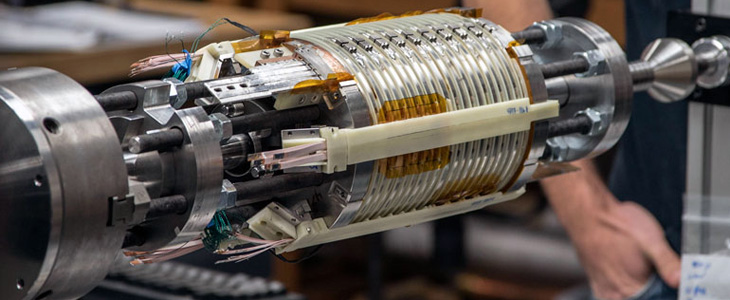
\includegraphics[width=15cm]{32_tesla_coil_730.jpg}
		\caption{The Natonal MagLab's 32-tesla all-superconducting magnet, featuring YBCO, under development. Image: Stephen Bilenky / National MagLab}
		
	\end{figure} 
	
	The above figure depicts the $32 T$ magnet developed at National MagLab opened up new realms for high energy particle accelerators. HTS magnet may also found substantial use in  fusion reactors. For such situations, the innovative design concept of remountable (or demountable) high-temperature superconducting (HTS) magnets have been proposed for both tokamak and helical reactors that use the HTS material features of high thermal stability and low cryogenic power \cite{TamuraHTSFusion}. They are already being used in NMR (Nuclear Magnetic Resonance) and MRI (Magnetic Resonance Imaging) techniques.
	
	\subsection{Applications in Power Electronics}
	
	High Temperature superconductors found profound application in Power application and Power industry. Low losses and high current density make them suitable for transmission lines, high critical field allows them to store magnetic field and thus useful in building strong magnets. These strong permanent magnets can be used in motors and generators and reduce power losses and improves efficiency. We look at these applications below in detail.
	\subsubsection{Cables / Wires}
	Various attempts are being made for residential HTS transmission cables. One such project is the \textit{Holbrook Superconductor Project} \cite{wikiCable} which installed HTS wire underground and chilled to superconducting temperature with liquid nitrogen.
	HTS cables are expected to have high current carrying
	capability, which could be interesting for retrofit of
	existing underground cables to increase transmission
	capacity in the same duct. With HTS cable, lower losses
	could be expected and, thus, design with lower voltage
	levels possible. However, the AC losses of available
	conductors are still too high, dielectric insulation at
	cryogenic temperatures (for designs with cold insulation) needs further understanding, and cable accessories
	(e.g. joints and terminations,) are still in the early stage of development. Above all, cooling systems with a high
	level of reliability and safety requiring a low number of
	cooling stations are yet to be demonstrated.
	
	\begin{figure}[h]
		\centering
		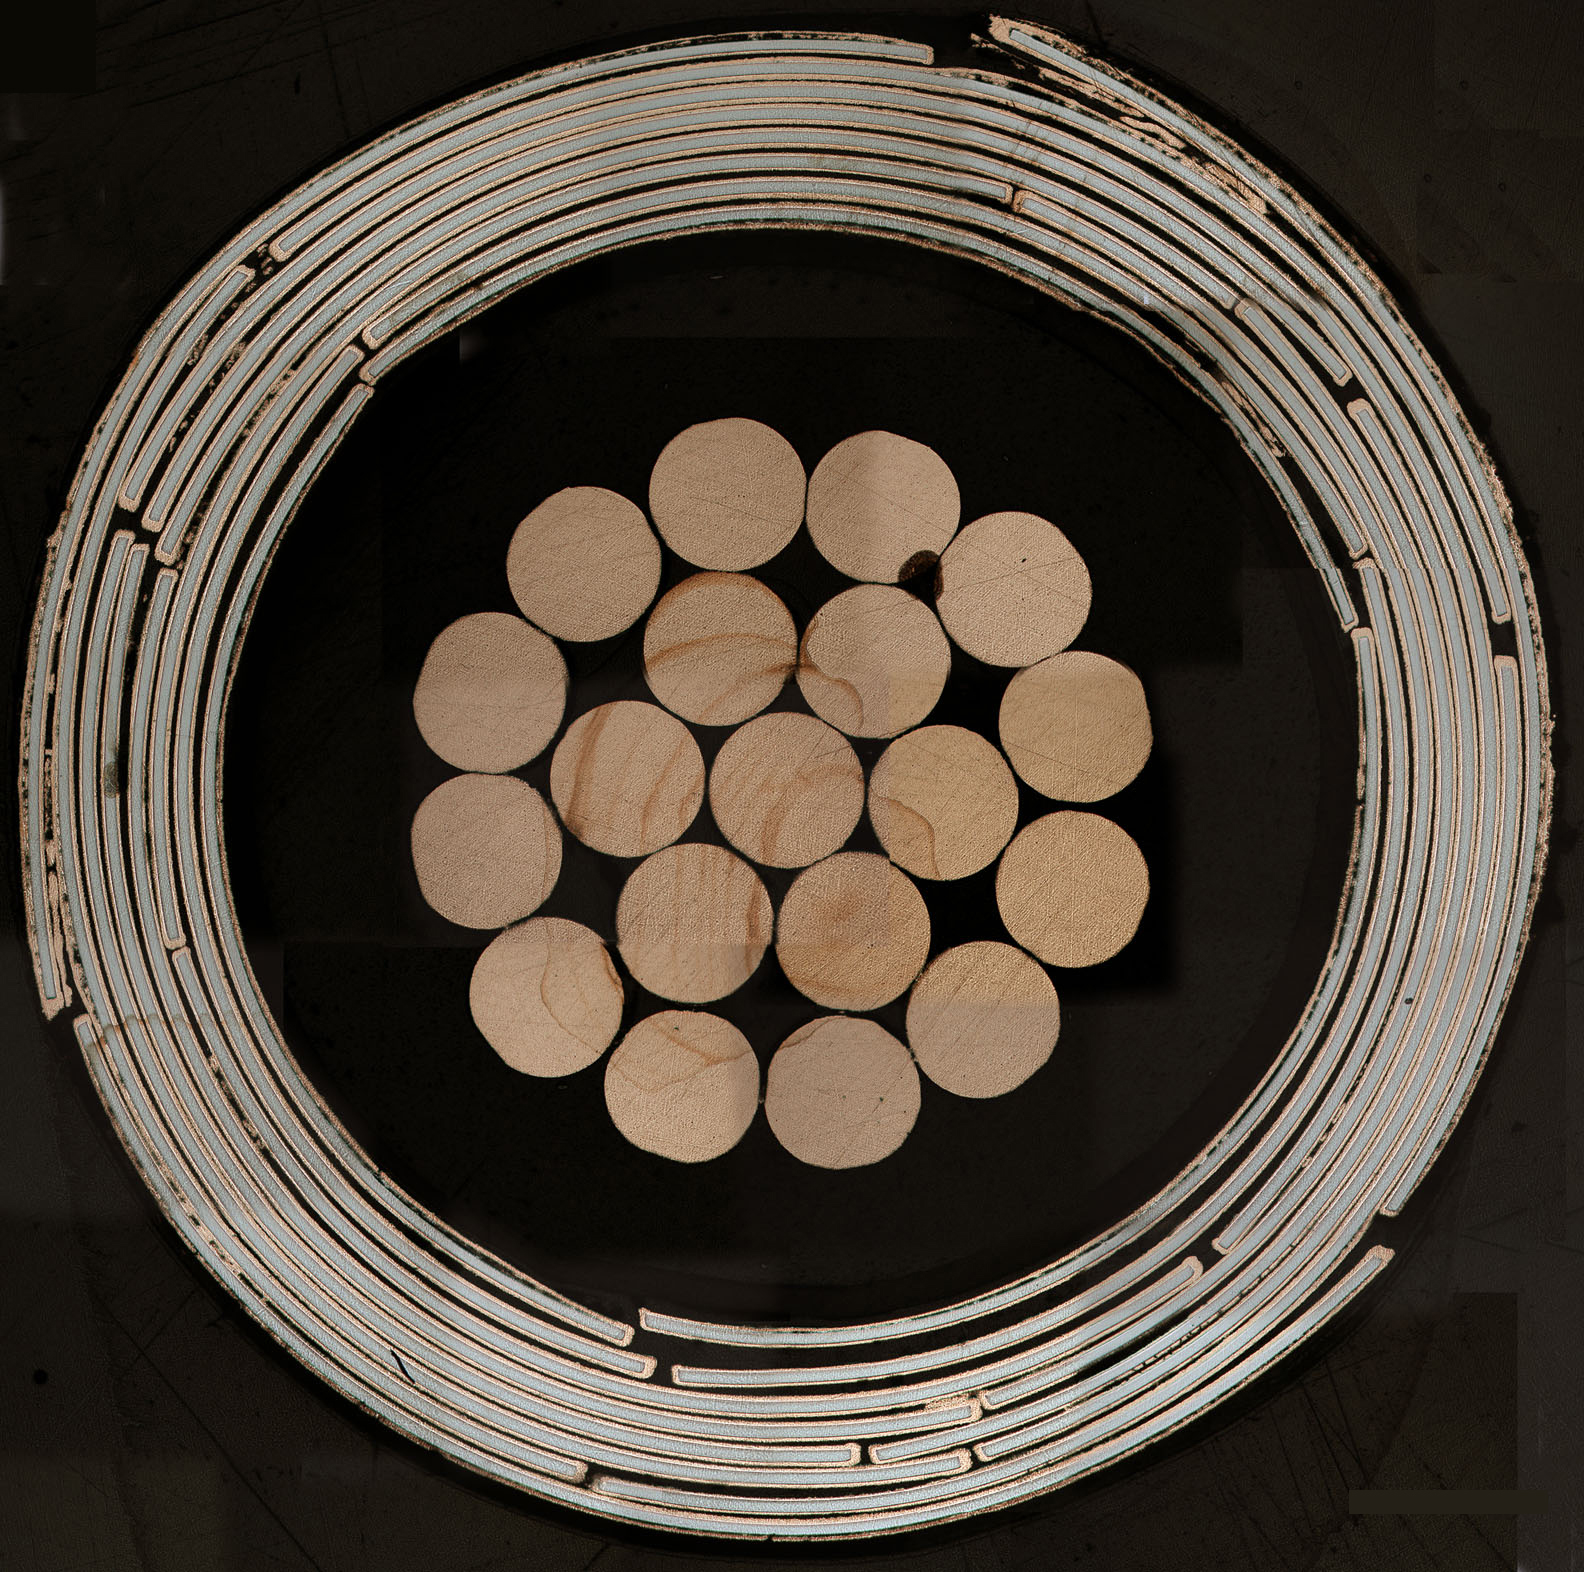
\includegraphics[width=5cm]{high_temperature_superconducting_cables.jpg}
		\caption{Cross-section of a high-temperature superconducting cable design invented at NIST. In the center are copper wires bundled with nylon and plastic insulation. The outer rings are a series of superconducting tapes wrapped in spirals around the copper. The cable is 7.5 mm in outer diameter. Credit: van der Laan/NIST }
		
	\end{figure} 
	
 \subsubsection{Transformers}
	
	With the improvement of high temperature superconductor (HTS), HTS transformers have been moving from the laboratory stage to industrial applications. A single-phase 2 MVA (66kV/6.9kV) prototype HTS transformer has been manufactured, tested and evaluated in 2005 is shown in Fig. 6 below \cite{hts2mva}.
	
	\begin{figure}[h]
		\centering
		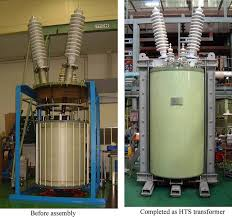
\includegraphics[width=5cm]{hts_transformer.jpeg}
		\caption{The 2 MVA HTS power transformer Source:  Xiaoyuan Chen et al., Journal of the European Ceramic Society  }
	\end{figure} 
	
	The major attraction for HTS Transformer lies in the potential for reduction (compared to conventional) in losses, volume, and weight. Furthermore, it offers overloadability without accelerated aging and possible integration of a fault current limitation function \cite{htspa}.
	\subsubsection{Motors}
	Rapid advances in the development of HTS
	wire over the past decades has resulted in HTS electromagnets that can operate at substantially higher temperatures than those made of Low temperature semiconductor materials, which poses advantage of relatively simple, less costly, and more efficient cryogenic systems.
	These factors enables HTS wires technically and economically viable for commercialization of motor and generator applications at significantly lower power ratings compared to LTS.
	
	\begin{figure}[h]
		\centering
		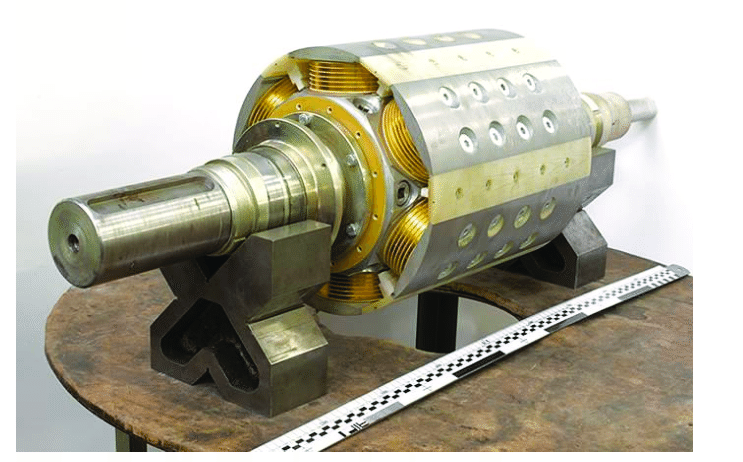
\includegraphics[width=5cm]{The-general-view-of-the-rotor-with-HTS-coils-of-the-200-kW-HTS-motor.png}
		\caption{The general view of the rotor with HTS coils of the 200 kW HTS motor. Source: V. P. Firsov et al. \cite{htsstator}}
		
	\end{figure} 
	
	The synchronous machine is the favorite choice for HTS motors. Most HTS machine employs superconducting field winding on the rotor, and a conventional copper winding on the stator. The potential benefits of an HTS motor are similar to that of HTS transformer. HTS motors provide high power density, high efficiency and low noise production. 
	
	\subsubsection{Fault Current Limiters}
	There are fair odds of short circuits in the power system and appliances. A large current flows during a short circuit and causes power loss and may damage appliances as well. Superconducting fault current limiters (SCFCL) remains in superconducting state and offers no resistance during the normal state of operation, and in the event of a fault, it reverts to normal state and reduces the current passively. 
	Superconducting    Fault Current Limiters (SCFCL) (see Fig. 8) could enable the novel design of electric grids. Most HTS FCL concepts exploit the sharp transition of superconductors from zero resistance, at normal currents, to finite resistance at higher current densities.
	\begin{figure}[h]
		\centering
		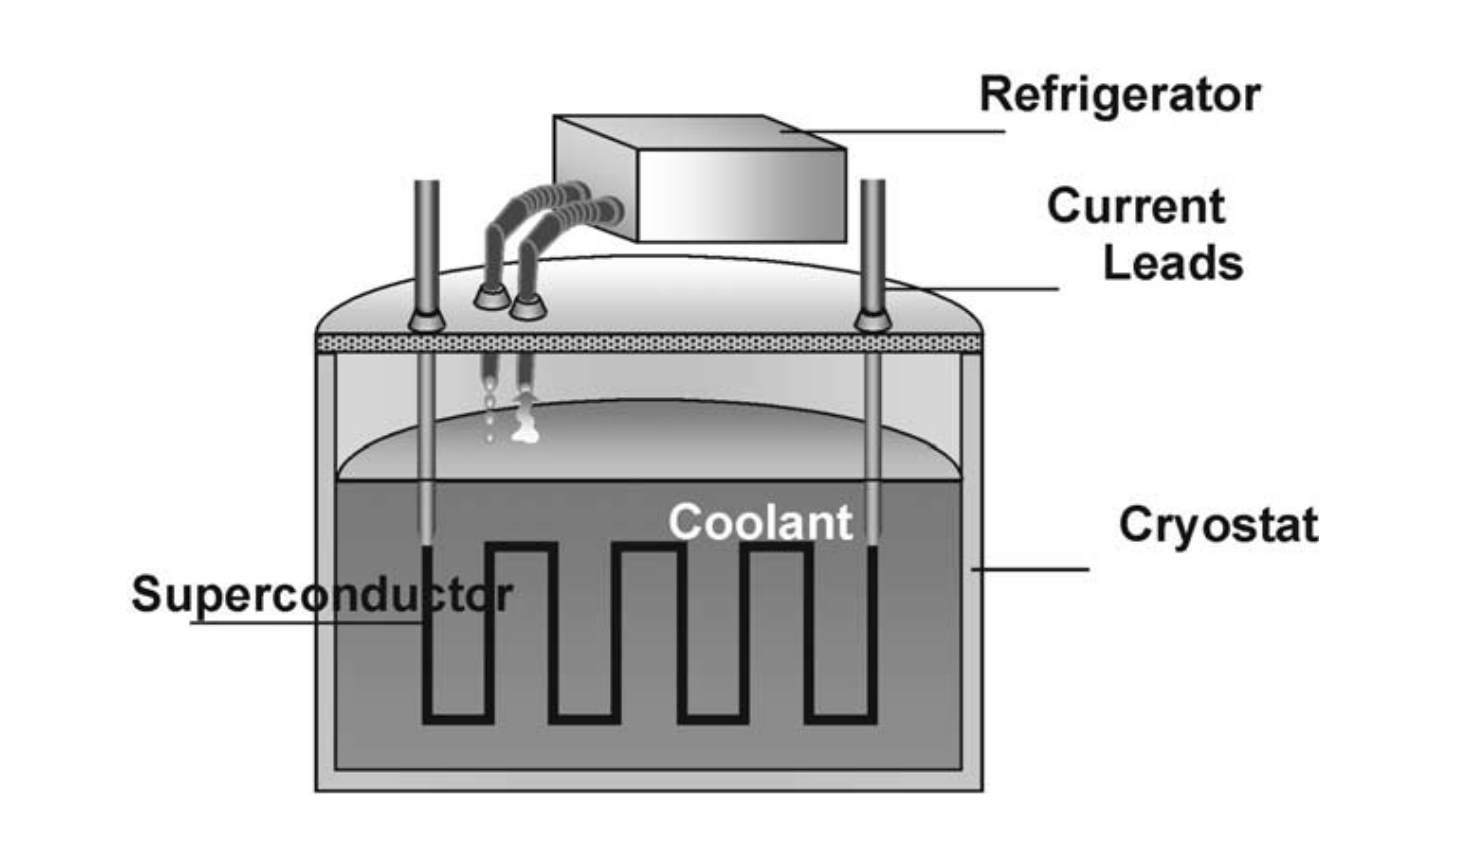
\includegraphics[width=10cm]{SCFL.png}
		\caption{Schematic drawing of a resistive superconducting fault current limiter with a closed cooling cycle, Willi Paul et al., ABB Switzerland, 2004 }
	\end{figure} 
	
	During normal operation, SCFCL operates with negligible impedance, and, in the event of fault current,
	SCFCL passively performs instantaneous limitation. It is an ideal fault current limiter and is exceptionally suited for grids with high prospective fault currents.
	Different high temperature superconductors (HTS) materials, like YBCO films, Bi2223 wires or Bi2212 bulk are under development for the use in SCFCL \cite{Lanz2001}. With SCFCL, it is possible to design grids with low impedance and improved power quality.
	
	\subsection{Applications in medical industry}
	Medical applications of superconductivity can be divided into two major categories. The first major category is based on the use of HTS powerful magnets, e.g., MRI and particle accelerators, and the second category is based on the detection of biomagnetism such as SQUID-based magnetoencephalography (MEG) and magnetocardiography (MCG) \cite{Hirano}.  The cost involved in manufacturing and maintaining HTS devices limit their medical applications. HTS technologies are quite costly for medical applications and limits to medical research institutes only. Medical industry faces criticism on high amount of medical bills when using HTS techniques.
	
	\subsection{Applications in Renewable Energy}
	One of the primary renewable energy source where HTS founds application is Wind energy. It is a clean source of energy but requires high capital investment. HTS wires and generators are profoundly used in Wind turbines. The enormous power density and high efficiency of HTS generators have been exploited for power generation in wind turbines. HTS generators are very powerful than conventional machines and ensure silent and smooth operation. Use of superconducting wire in the windings allows for very slow speed generators, and high currents without losses, and removes large mechanical gearboxes which in turn increases the speed and mechanical losses. Incorporating zero-resistance, HTS wires boost efficiency and lead to smaller, lighter turbines which are also easier to transport, install and maintain.
	
	\begin{figure}[h]
		\centering
		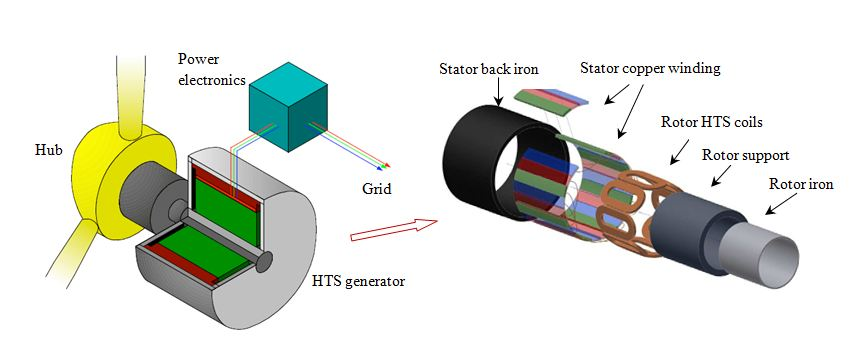
\includegraphics[width=10cm]{hts_wind_turbine.jpeg}
		\caption{Schematic of a HTS synchronous generator system \textbf{Source}: \href{https://www.intechopen.com/books/advances-in-wind-power/wind-turbine-generator-technologies}{Zheng Tan et al.}}
	\end{figure}
	
	\paragraph{}
	One of the major challenges faced by the renewable energy industry is the storage of generated energy. During the peak hours all of the generated energy is used whereas during night time this usage reduces drastically but the generation of electrical energy may continue (E.g., Wind velocity increases during the night and produces a large amount of energy). Storage of this energy is crucial to the success of renewable sources. The energy stored in the form of magnetic field in High Temperature Superconductors facilitates the storage of electrical energy. Renewable energy can be immensely benefited from HTS as it minimises losses and improves efficiency. This requires further development of HTS wire current carrying capabilities, cryogenic systems, cooling stations and power electronics.
	
	\section{Future Research}
	We have successfully built prototypes for various applications of High Temperature Semiconductors, but we are yet far from their commercialization because we still don't know how superconductivity arises in High Temperature Semiconductors. The cause behind the formation of pairs of electrons in these crystals is not known yet\cite{Legget}. HTS has a great analogy with neural networks, i.e. we have started using them for a large number of applications But we still don't know its working. Commercialization of existing applications needs to be investigated further and cooling stations \& mechanisms needs to be developed.
	\section{Conclusion}
	High temperature semiconductors have already developed to the point that many commercial applications are in place. With the bleeding edge of research, we are delving deeper into High Temperature superconductivity and trying to understand its cause. The mystery behind the formation of electron pairs will definitely fetch a Nobel Prize. Room temperature superconductors with desired materials will allow us to commercialize scientific prototypes and open new avenues. 
	
	
	\bibliographystyle{unsrt}  
	%\bibliography{references}  %%% Remove comment to use the external .bib file (using bibtex).
	%%% and comment out the ``thebibliography'' section.
	
	
	%%% Comment out this section when you \bibliography{references} is enabled.
	\begin{thebibliography}{1}
		
		
		\bibitem{HTSdevices}
		\newblock Seeber, B., Handbook of Applied Superconductivity. IOP Publishing, Bristol, 1998.
		
		\bibitem{HTSmotor}
		\newblock Madura, D., et al., Test results of a 5000hp HTS motor. IEEE Trans. Appl. Superconductivity, presented at ASC 2002, (in press).
		
		\bibitem{SCFCL}
		\newblock Paul, W., et al., Test of 1.2 MVA High-Tc Superconducting Fault Current Limiter. Superconducting Science and Technology, 1997, 10, 914–918.
		
		\bibitem{HTStransformer}
		\newblock Therond, P. G. et al., High Temperature 630 kVA Super-conducting Transformer. CIGRE, 1998, 12–302.
		
		\bibitem{powercable}
		\newblock Stovall, J. P. et al., Operating experience with the Southwire 30-meter high-temperature superconducting power cable. Adv. Cryog. Eng., 2002, 47, 591.
		
		\bibitem{highestTc}
		A. P. Drozdov1, P.P. Kong, V.S. Minkov, S.P.Besedin, M.A. Kuzovnikov1, S. Mozaffari, L. Balicas, F. Balakirev, D. Graf, V. B. Prakapenka, E. Greenberg, D. A. Knyazev, M. Tkacz, and M.I.Eremets.
		\newblock Superconductivity at 250 K in lanthanum hydride under high pressures
		
		
		\bibitem{criticalfieldform}
		\newblock High Temperature Superconductivity, Jeffrey W. Lynn Editor, Springer-Verlag (1990)
		
		\bibitem{ceramicsbarrier}
		\newblock L. R. Lawrence et al: "High Temperature Superconductivity: The Products and their Benefits" Archived 2014-09-08 at the Wayback Machine (2002) Bob Lawrence \& Associates, Inc.
		
		\bibitem{noblePress}
		\newblock Press release: The Nobel Prize in Physics 2016., The Royal Swedish Academy of Sciences, \href{https://www.nobelprize.org/uploads/2018/06/advanced-physicsprize2016.pdf}{https://www.nobelprize.org/uploads/2018/06/advanced-physicsprize2016.pdf}
		
		
		\bibitem{htspm}
		\newblock Nariki, S., Sakai, N. \& Murakami, M. Processing of high-performance Gd-Ba-Cu-O bulk
		superconductor with Ag addition. Supercond. Sci. Technol. 15, 648–652 (2002).
		
		\bibitem{saleem2014}
		\newblock Iqbal and Saleem, J Bioeng Biomed Sci 2014, 4:1., A Perspective on Medical Applications of High Temperature Superconductors
		
		\bibitem{TamuraHTSFusion}
		\newblock Satoshi Ito, Hidetoshi Hashizume, Nagato Yanagi, Hitoshi Tamura, Advanced high-temperature superconducting magnet for fusion reactors: Segment fabrication and joint technique
		
		\bibitem{wikiCable}
		\newblock Gelsi, Steve (2008-07-10). "Power firms grasp new tech for aging grid". Market Watch. Retrieved 2008-07-11.
		
		\bibitem{hts2mva}
		\newblock T. Bohno, A. Tomioka, M. Imaizumi, Y. Sanuki, T. Yamamoto, Y. Yasukawa, H. Ono, Y. Yagi, and K. Iwadate, “Development of 66 kV/6.9 kV 2 MVA prototype HTS power transformer,” Physica C, vol. 426–431, pp. 1402–1407, 2005
		
		\bibitem{htspa}
		\newblock Makan Chen, Lise Donzel, Martin Lakner, Willi Paul, High temperature superconductors for power applications, Journal of the European Ceramic Society 24 (2004) 1815–1822
		
		\bibitem{htsstator}
		\newblock S Dezhin, Konstantin Kovalev, L G Verzhbitskiy,V. P. Firsov.,  Design and Testing of 200 kW Synchronous Motor with 2G HTS Field Coils, IOP Conference Series Earth and Environmental Science 87(3):032007
		
		\bibitem{Lanz2001}
		\newblock W. Paul, M. Chen, M. Lakner, J. Rhyner, D. Braun, W. Lanz., Fault current limiter based on high temperature    superconductors - different concepts, test results, simulations, applications
		
		\bibitem{Legget}
		\newblock A. Leggett (2006). "What DO we know about high Tc?". Nature Physics.
		
		\bibitem{Hirano}
		\newblock Takahashi H, Igawa K, Arii K, Kamihara Y, Hirano M, et al. (2008) Superconductivity at 43 K in an iron-based layered compound LaO1-
		xFxFeAs. Nature 453: 376-378.
	\end{thebibliography}
	
	
\end{document}


